%%%%%%%%%%%%%%%%%%%%%%%%%%%%%%%%%%%%%%%%%%%%%%%%%%%%%%%%%%%%%%%%%%%%
% Authors: A. Herrera-Poyatos, F. Herrera
% Tittle: Algoritmo memético equilibrado con diversificación voraz
% 							 CAEPIA 2015
%%%%%%%%%%%%%%%%%%%%%%%%%%%%%%%%%%%%%%%%%%%%%%%%%%%%%%%%%%%%%%%%%%%%

\section{Conclusión}

	\begin{frame}{Conclusiones: AMEDV}
		\begin{itemize}
			\item La diversificación voraz permite resolver el problema de la diversidad en la población de los algoritmos meméticos.
			\item El buen comportamiento del algoritmo pone de manifiesto la necesidad de mantener la diversidad de la población en los algoritmos meméticos así como como conseguir el aprovechamiento de la misma mediante el resto de operadores del algoritmo.
		\end{itemize}
		
		\begin{tcolorbox}[colback=blue!5,colframe=blue!30]
			\centering
			\color{blue!80} \textbf{El equilibrio entre exploración y explotación es esencial para el buen funcionamiento del algoritmo.}
		\end{tcolorbox}
	\end{frame}

	\setbeamertemplate{headline}{
		\begin{beamercolorbox}[wd=\paperwidth,ht=5pt]{last head}
		\end{beamercolorbox}

		\begin{beamercolorbox}[sep=4pt]{title} 
			\usebeamerfont{title} \color{white} Gracias por su atención.
		\end{beamercolorbox}
	}
	\usebackgroundtemplate{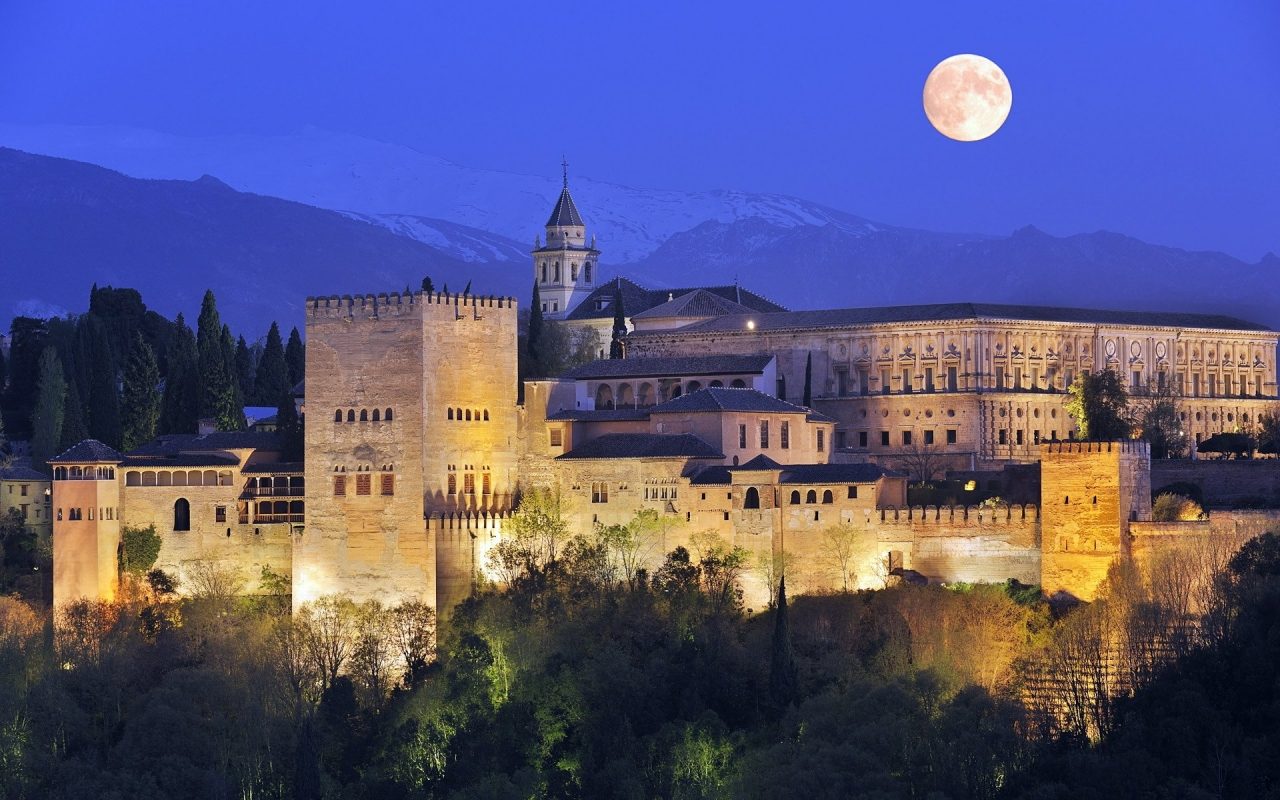
\includegraphics[height=0.9\paperheight,width=\paperwidth]{./Images/Wallpapers/alhambra.jpg}}

	\begin{frame}
	
	\end{frame}
	